\documentclass[11pt,svgnames,fontset=fandol]{ctexrep}
\usepackage[tt=false,osf]{libertine}
\usepackage[
    hmargin=2cm,
    vmargin=3cm,
    a4paper,
]{geometry}

\usepackage{framed}
\newcommand\mybullet[1]{\noindent\textbullet\;\textbf{\large #1}}
\AddToHook{env/leftbar/begin}{\par\setlength{\parindent}{0pt}}

\pagestyle{plain}
% \usepackage[cachedir=.]{luadraw}
% \usepackage{fancyhdr}
% \pagestyle{fancy}
% % https://tex.stackexchange.com/a/760676/322482
% \begin{luacode*}
% function do_cfoot()
%     local n = tex.count['c@page']
%     local g = graph:new{window={-5,5,-5,5},margin={0,0,0,0},size={1.2,1.2}}
%     local steps = math.min(n, 30)
%     for k = 1, steps do
%         local col = palette(rainbow, k/steps)
%         g:Filloptions("full", col, 0.25)
%         g:Dpolyreg(0, 3.5, 6, "draw=none,opacity=0.5,rounded corners=.5pt")
%         g:Rotate(12)
%         g:Scale(0.93)
%     end
%     g:IDmatrix()
%     g:Dlabel("\\bfseries\\color{black} " .. n, 0, {pos="center",node_options="text=black,opacity=1"})
%     g:Sendtotex()
% end
% \end{luacode*}
% \cfoot{\directlua{do_cfoot()}}
% \fancypagestyle{plain}[fancy]{}

% https://github.com/OsbertWang/install-latex-guide-zh-cn/blob/master/install-latex-guide-zh-cn.tex#L3-L11
\ctexset{
  chapter        = {
    format       = \huge\bfseries\raggedright,
    number       = \arabic{chapter},
    beforeskip   = 20pt,
    afterskip    = 15pt,
    name         = {},
    break        = {},
  },
}

\usepackage{hyperref}
\hypersetup{
  colorlinks=true,
  linkcolor=blue,
  urlcolor=red!70!black,
  citecolor=blue
}

\usepackage{graphicx}

\usepackage{listings, fancyvrb}
\lstset{
  breaklines      = true,
  columns         = fullflexible,
  showstringspaces= false,
  tabsize         = 4,
  gobble          = 1,
  numbers         = left,
  numberstyle     = \tiny\ttfamily,
  numbersep       = \ccwd,
  frame           = lines,
  rulecolor       = \color{blue!40},
  backgroundcolor = \color{lightgray!20},
  language        = bash,
  alsoletter      = -,
  basicstyle      = \small\ttfamily,
  commentstyle    = \color{olive!80!black},
  stringstyle     = \color{brown},
  emph            = { bash, cd, cp, dpkg, find, grep, ln, md5sum, mkdir,
                      mount, rm, rmdir, set, sha512sum, sudo, umount },
  emphstyle       = \color{blue}\bfseries,
  morekeywords    = { add-apt-repository, apt, brew, certutil, evince,
                      fc-cache, fc-list, fmtutil, fmtutil-user, fmtutil-sys,
                      gedit, kpsewhich, l3build, latexmk, mkfontdir,
                      mkfontscale, notepad, tex, texdoc, tlmgr, pdflatex,
                      visudo, wget, wsl, xelatex },
  keywordstyle    = \color{teal}\bfseries
}
\lstdefinelanguage{json}{
  basicstyle   = \small\ttfamily\color{DarkBlue},
  numberstyle  = \tiny\ttfamily\color{black},
  alsoletter   = ",
  morecomment  = [l]{//},
  morekeywords = {"latexmk", "latexmkpdf", "latexmkxe", "never", "tab", "external"},
  keywordstyle = \color{FireBrick}\bfseries,
  literate     ={*[{\textcolor{DarkGreen}{[ }}1  ]{\textcolor{DarkGreen}{ ]}}1
                 \{{\textcolor{DarkRed}  {\{}}1 \}{\textcolor{DarkRed}  {\}}}1
                  :{\textcolor{black}    {:}} 1  ,{\textcolor{black}    {,}} 1}
}
\lstdefinelanguage{mwe}{
  language     = {[LaTeX]TeX},
  texcsstyle   = *\color{violet},
  morekeywords = {article, ctexart, document},
  literate     =*\{{\textcolor{magenta}\{}1 \}{\textcolor{magenta}\}}1
}

\usepackage{tcolorbox}
\tcbuselibrary{listings,skins}

\newtcolorbox{examplecode}{
  colback=white,
  colframe=white,
  leftrule=0pt,
  rightrule=0pt,
  toprule=0pt,
  bottomrule=0pt,
  boxrule=0pt,
  arc=0pt,
  borderline west={2pt}{0pt}{red},
  borderline east={2pt}{0pt}{orange},
  borderline north={2pt}{0pt}{violet},
  borderline south={2pt}{0pt}{blue},
  left=1em,
  right=1em,
  top=0.5em,
  bottom=0.5em,
}

\newtcolorbox{featurebox}{
  colback=gray!5,
  colframe=gray!50,
  boxrule=0.5pt,
  arc=2pt,
  left=1em,
  right=1em,
  top=0.5em,
  bottom=0.5em,
}

\usepackage{enumitem}
\setlist{nosep, leftmargin=2em}

\begin{document}

\begin{center}
  {\Large\bfseries Vscode+LaTeX Workshop+TeXLive配置指南}—v1.1
\end{center}

\begin{flushright}
  {\large Explorer \hspace{.5em} 2025-03-14}
\end{flushright}

本文将从一名萌新的视角出发，介绍如何一步步顺利在vscode中配置LaTeX Workshop的设置，并顺利编译出你的第一份PDF文件.

\chapter{命令行编译}

可能有的人会说，作为萌新用户，并不需要掌握命令行编译，或者更有甚者看到需要在「一个黑色框中手动输入代码」就会感到害怕. 事实上，这种看法在我看来是较为片面的，要想真正用好TeXLive，\textbf{必须先掌握「命令行编译」}.

此事在\textbf{优秀的安装教程}\href{https://github.com/OsbertWang/install-latex-guide-zh-cn}{install-latex-guide-zh-cn}的第一章中亦有记载，在顺利安装完TeXLive之后，首要的便是掌握「命令行编译」.

首先相信每位读到本文的用户面前肯定已经打开了一个\texttt{.tex}文件，它可能是「2077年全国大学生数学竞赛模板」、或者是「广为流传的\href{https://github.com/ElegantLaTeX/ElegantBook}{\texttt{elegantbook}系列模板}」，如果你还没有配置好vscode的编译环境，请先\textbf{关闭这些较为复杂的模板}，从下面这个「最简单」的例子开始.

\textbf{罗马不是一天建成的}，还没学走路就想飞，只会在配置的过程中遇到更多的问题，最终因为配置和 debug 极其麻烦而更容易打退堂鼓.

\textbf{工欲善其事，必先利其器。} 在这里有必要顺便强调一下「\textbf{编辑器}」和「\textbf{编译器}」的区别.

\begin{itemize}
  \item \textbf{编辑器（editor）}只不过是用来「编辑文本」的，我们这里用到的\texttt{vscode}就是这样的工具，它并没有任何编译功能. 使用「\texttt{vscode}」编写程序和使用「记事本（\texttt{notepad}）」编写程序从其本质来看是没有任何区别的.
  \item \textbf{编译器（compiler）}才是真正用来「把代码转换成PDF」的工具. 这里我们使用的编译器是\texttt{TeXLive}，它是一个非常庞大的编译器集合，里面包含了各种各样的编译器. 注意，你大致可以把编译器理解为「可执行程序（e.g. \texttt{Genshin Impact.exe}）」，这类程序执行的时候，会按照其内部逻辑处理你的代码，并根据程序设定好的功能执行任务.
\end{itemize}

一言以蔽之，我们在这里要实现的，是用「vscode」作为代码\textbf{编辑器}来编写代码，并调用我们目标的\textbf{编译器}（这里是\texttt{TeXLive}中的\texttt{pdflatex.exe}、\texttt{luatex.exe}等），通过这些程序将我们编写的代码转换成目标的PDF文件.

如果你已经仔细阅读了\href{https://github.com/OsbertWang/install-latex-guide-zh-cn}{install-latex-guide-zh-cn}并且顺利安装了TeXLive，此时在终端中输入\texttt{xelatex -v}，理应看到类似如下的终端输出:

\begin{lstlisting}[language=bash]
$ xelatex -v
XeTeX 3.141592653-2.6-0.999997 (TeX Live 2025)
kpathsea version 6.4.1
Copyright 2025 SIL International, Jonathan Kew and Khaled Hosny.
There is NO warranty.  Redistribution of this software is
covered by the terms of both the XeTeX copyright and
the Lesser GNU General Public License.
For more information about these matters, see the file
named COPYING and the XeTeX source.
Primary author of XeTeX: Jonathan Kew.
Compiled with ICU version 76.1; using 76.1
Compiled with zlib version 1.3.1; using 1.3.1
Compiled with FreeType2 version 2.13.3; using 2.13.3
Compiled with Graphite2 version 1.3.14; using 1.3.14
Compiled with HarfBuzz version 10.2.0; using 10.2.0
Compiled with libpng version 1.6.46; using 1.6.46
Compiled with pplib version v2.2
Compiled with fontconfig version 2.15.0; using 2.15.0
\end{lstlisting}

废话有点多，我们先来用「命令行编译」第一个\texttt{.tex}文件:

首先在系统中的某处新建一个文件夹，并且右键新建一个\texttt{.tex}文件（可以新建一个文本文档，再将后缀名\texttt{.txt}修改为\texttt{.tex}）. 如果文件资源管理器默认没有显示后缀名，则自行通过搜索引擎检索如何调出来.\\
注意，虽然现在已经是2025年了，但还是\textbf{极其不建议}用户使用「中文文件名」、「带空格的路径」. 请用「\texttt{main.tex}」而不是「\texttt{我的模板 哈哈哈.tex}」. 后者既有中文，又有空格，真是\textbf{坏透了}. 之后在这个\texttt{.tex}所在的文件夹内，在空白区域处右键后点击「在终端中打开」或「通过\texttt{Code}打开」:

\begin{center}
  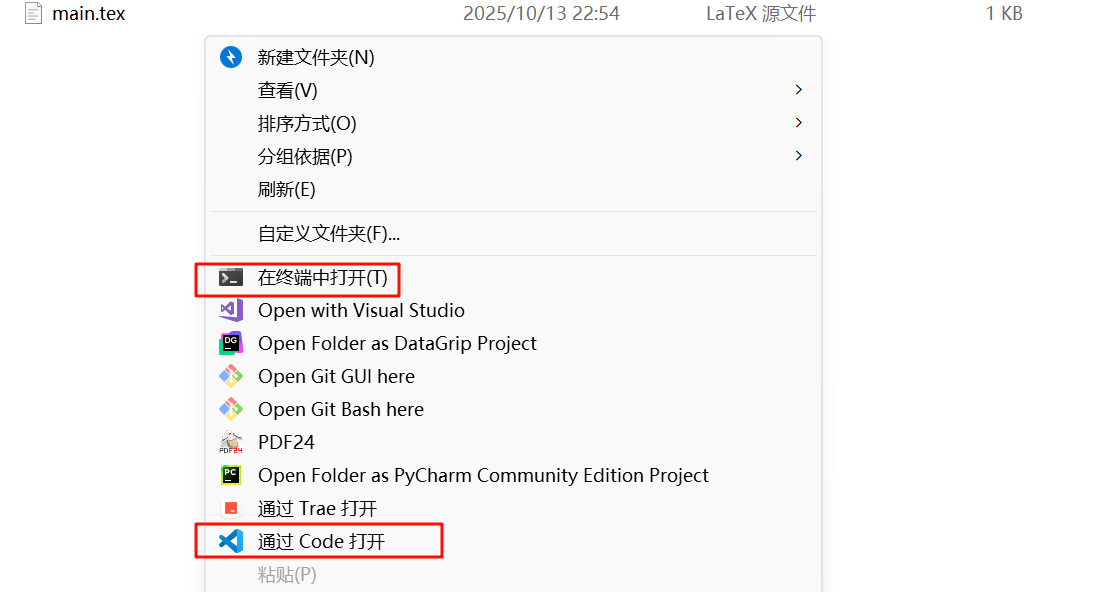
\includegraphics[width=\textwidth]{open-terminal.png}
\end{center}

如果找不到这两项，那么也请自行通过搜索引擎检索如何把它们调出来. 这里采用「通过Code打开」作为示例，如果你不能看到下方的「Terminal」面板，可以通过快捷键「Ctrl+\`」呼出.

并且把下面这一「最小工作示例」的「\texttt{Hello, World!}」文件复制到\texttt{.tex}文件中：

% \begin{examplecode}
\begin{lstlisting}[language=TeX]
\documentclass{ctexart}
\begin{document}
Hello, World!

你好, \LaTeX{}！
\end{document}
\end{lstlisting}
% \end{examplecode}

\begin{center}
  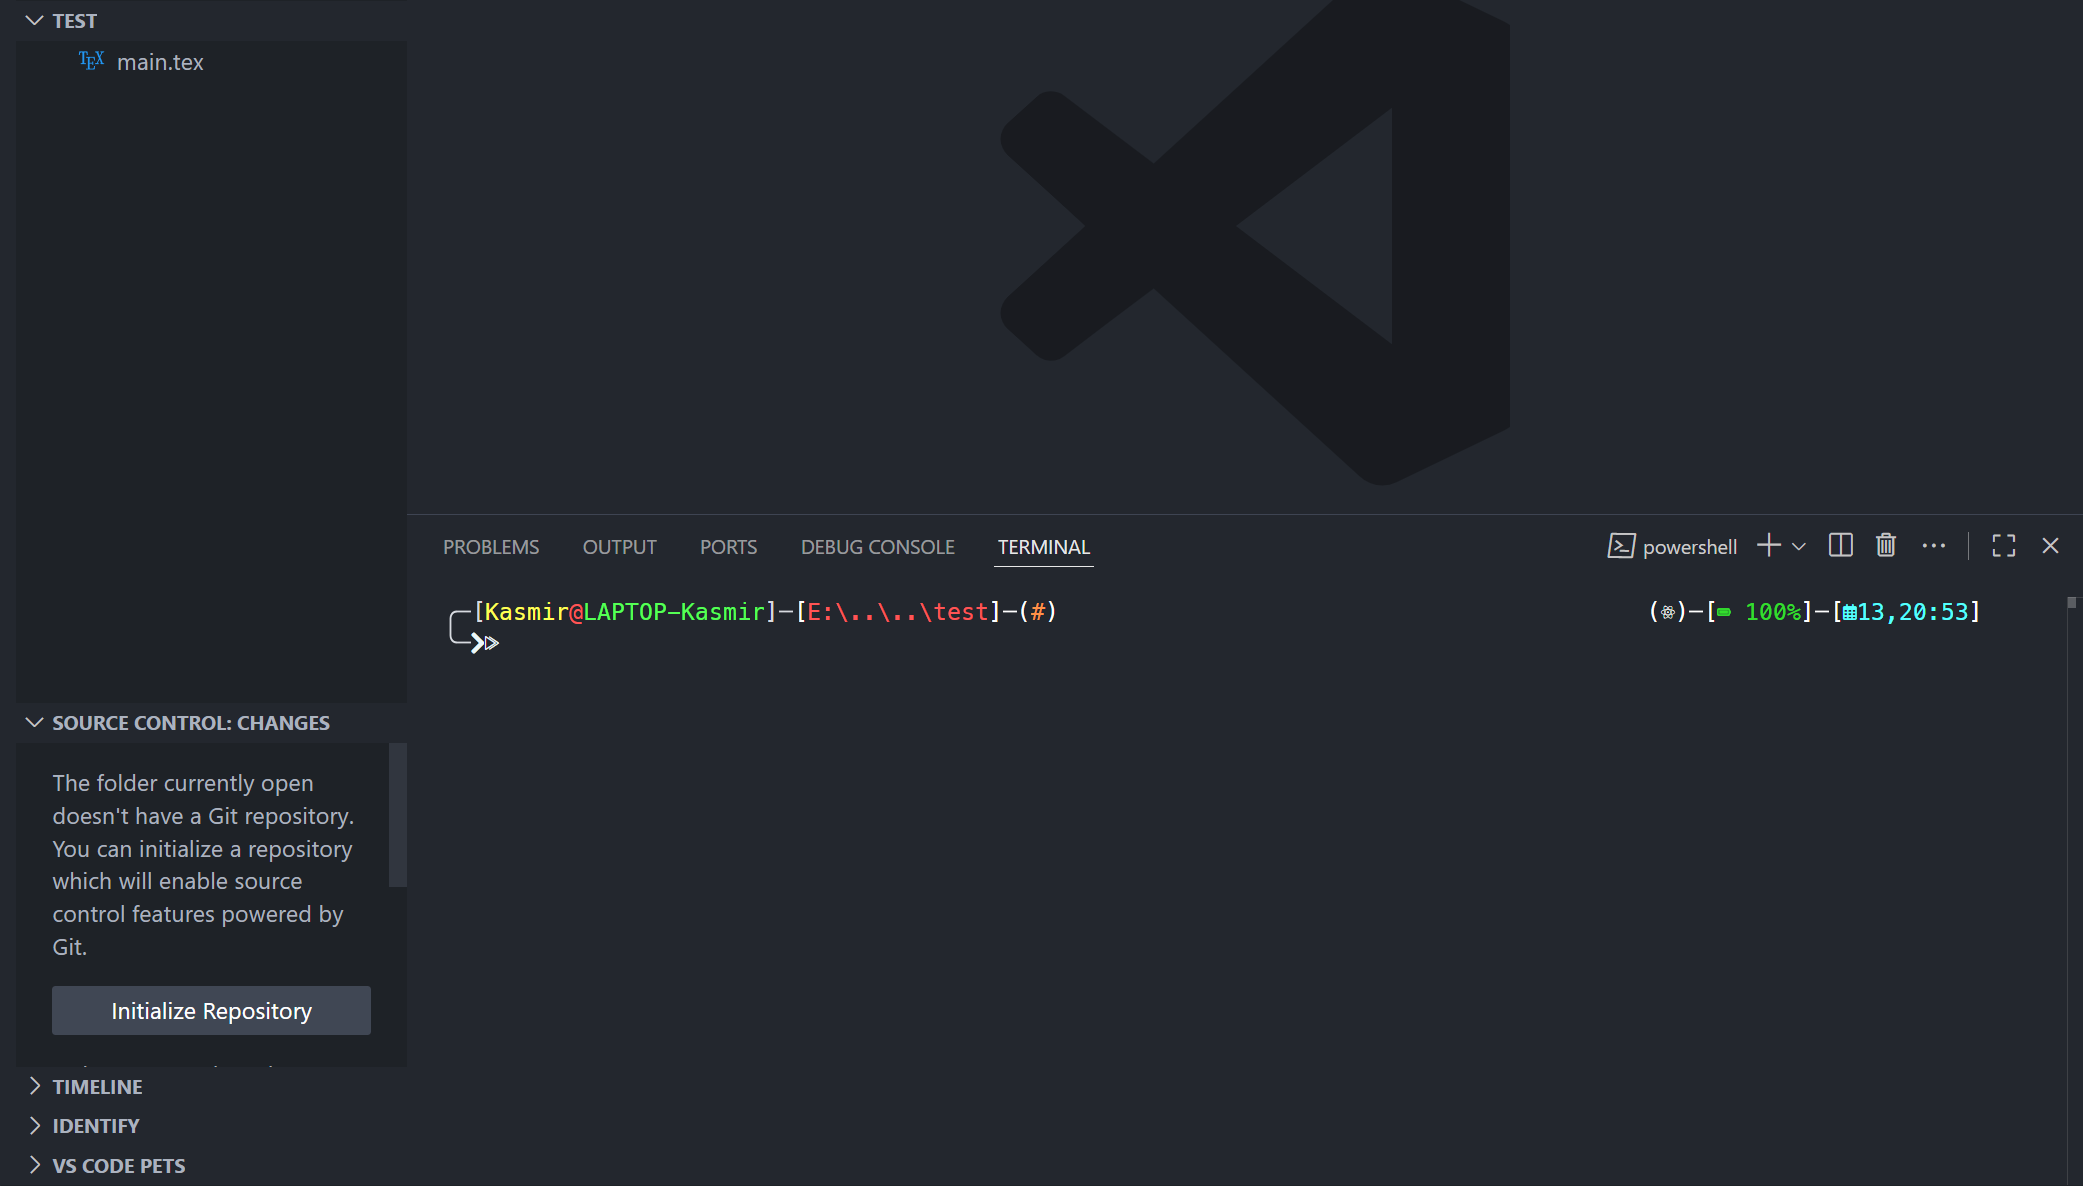
\includegraphics[width=\textwidth]{vscode-terminal.png}
\end{center}

在vscode的终端中，注意到当前所在的路径「\texttt{E:\textbackslash..\textbackslash..\textbackslash test}」恰好是我们新建的\texttt{main.tex}所在的路径，这就免去了切换到工作路径的繁琐. 此时在「Terminal」中输入:

% \begin{examplecode}
\begin{lstlisting}[language=bash]
xelatex main.tex
\end{lstlisting}
% \end{examplecode}

并回车, 我们预期可以看到这样的场景:

\begin{center}
  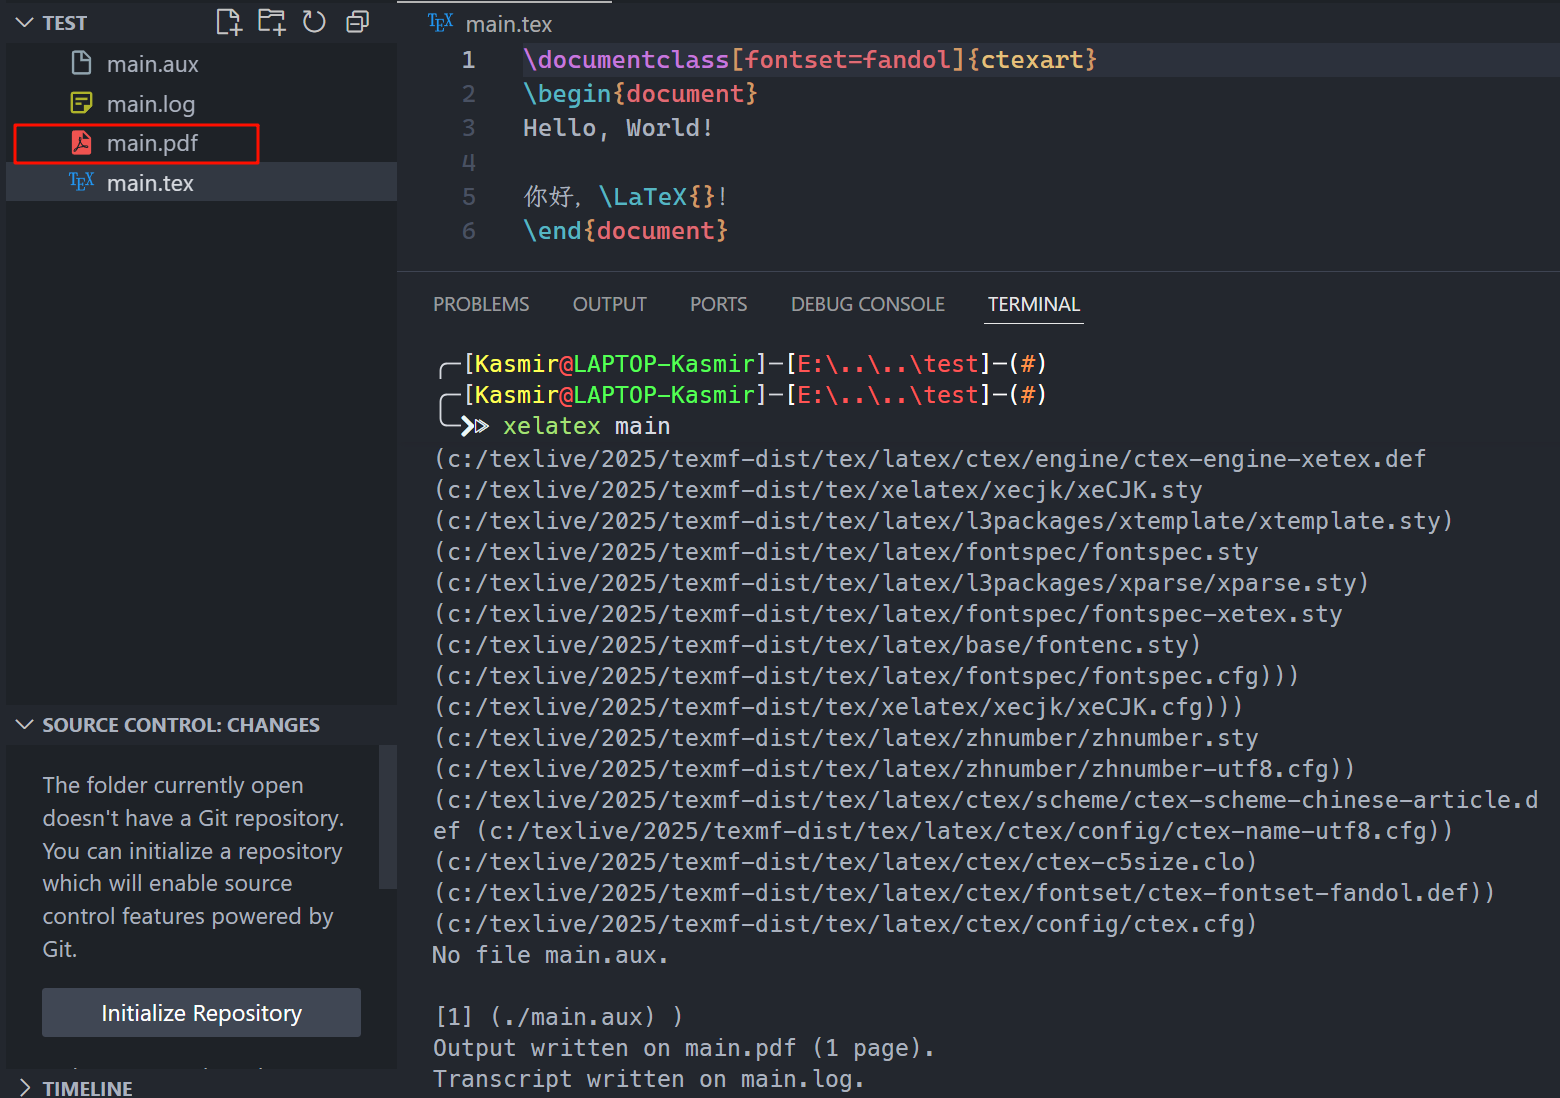
\includegraphics[width=\textwidth]{compiling.png}
\end{center}

注意到左侧边栏文件夹处出现了一个名为「\texttt{main.pdf}」的文件，这便是我们第一次编译顺利完成的标志. 单击打开，我们可以看到编译的结果.

\chapter{使用 LaTeX Workshop 插件辅助编译}

洋洋洒洒，我们却还没有进入真正的主题——\textbf{L}\textit{a}\textbf{TeX} \textbf{W}\textit{orkshop}(\textbf{LW}) 插件. 但事实上，我们已经手动实现了编译，并且得到了最终的PDF文件，这就对了！事实上，要想编译一个\texttt{.tex}文件，我们\textit{并不需要}「LaTeX Workshop」！\\
那么为什么互联网上铺天盖地的文章都在用呢？是因为这个插件实际上只是在帮助我们\textbf{自动做}「手动打开终端-根据文件名输入\texttt{xelatex main.tex}」这件事而已（设想如果文件名很长，每次都需要手动输入\texttt{pdflatex wileyNJDv5\_AMA.tex}会显得尤为繁琐）. 同时由于配置较为复杂，因此常常成为萌新用户的拦路虎.

首先我们要安装「LaTeX Workshop」插件.

\begin{center}
  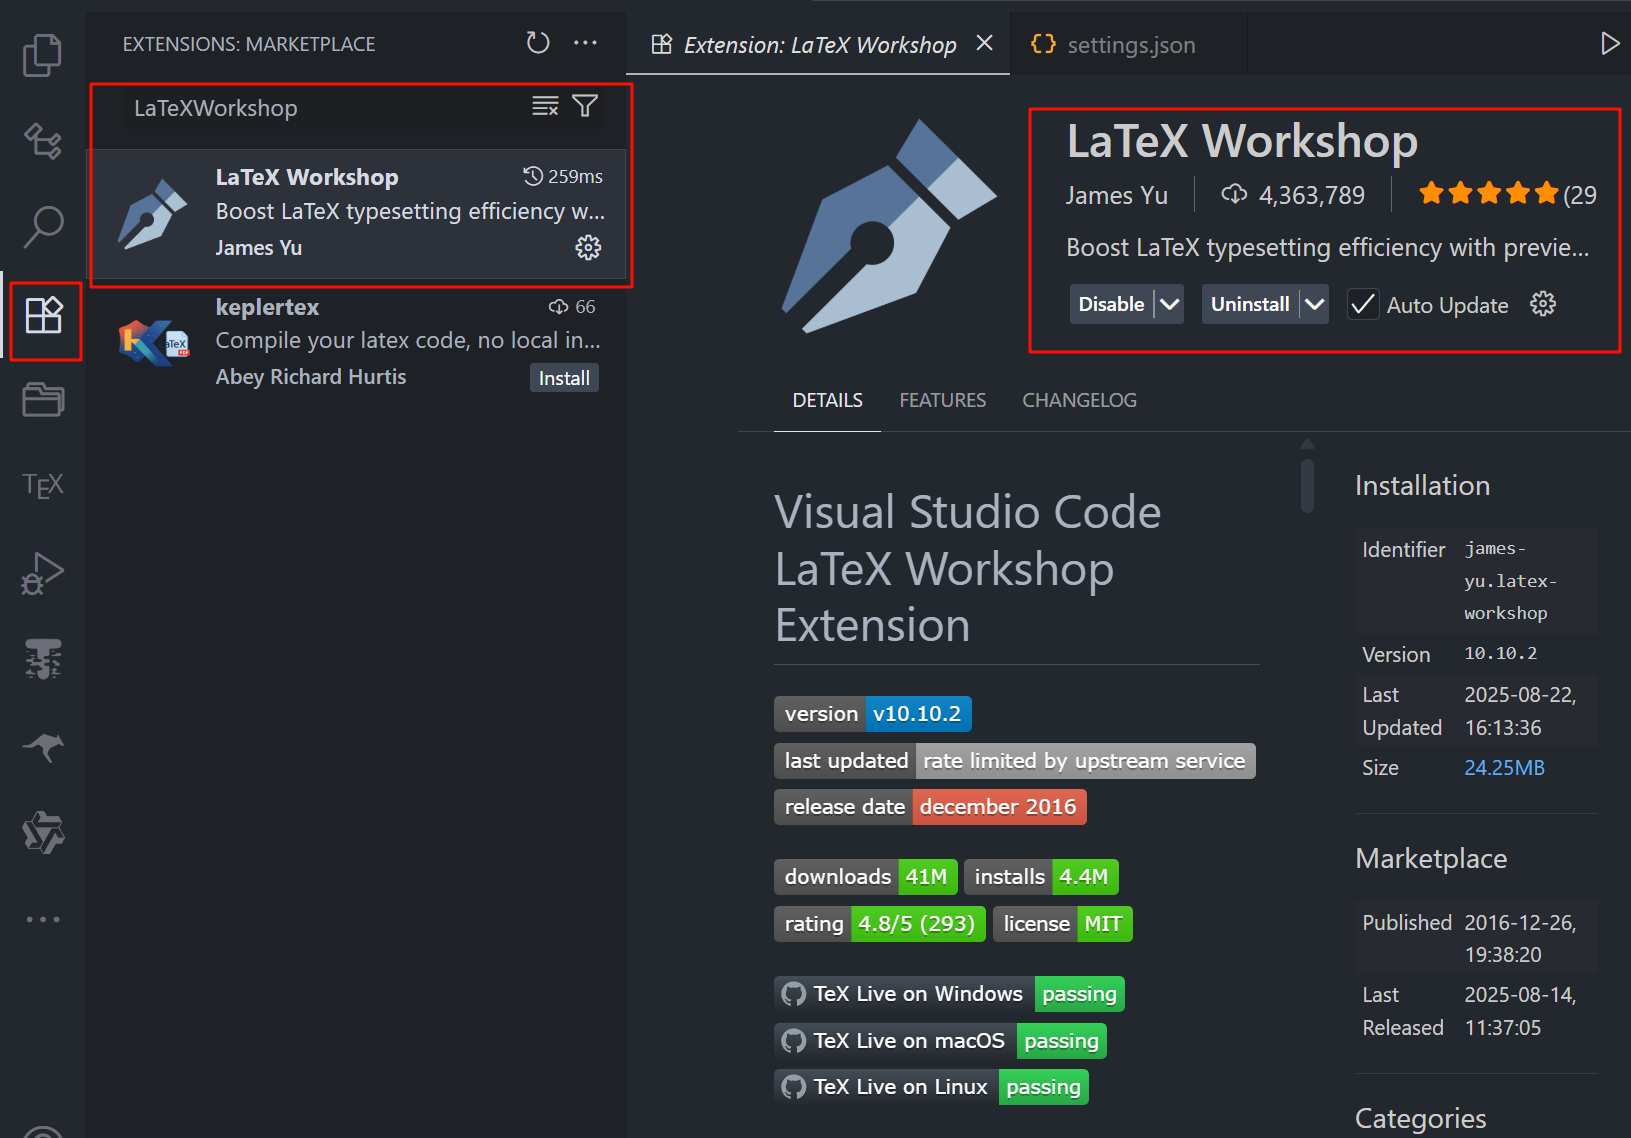
\includegraphics[width=0.925\textwidth]{LW-install.png}
\end{center}

安装插件之后，只有\textbf{当你创建并打开了一个\texttt{.tex}文件的时候}，左侧边栏才会出现「TeX图标」

\begin{center}
  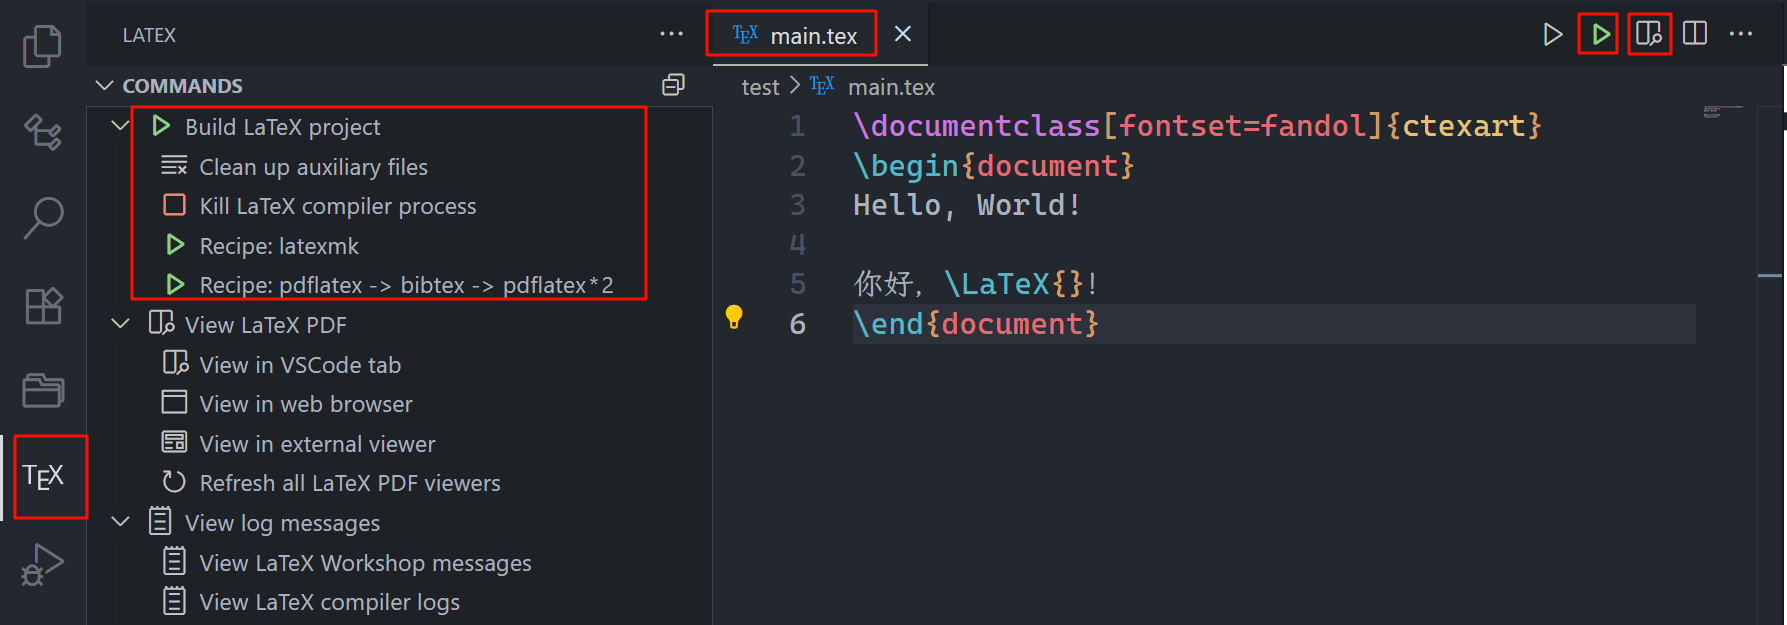
\includegraphics[width=0.95\textwidth]{TeX-panel.png}
\end{center}

注意上图中圈出来的按钮，分别可以实现「选择不同的编译工具」、「快速编译」、「预览PDF文件」等功能. 当然，左侧边中还提供了形如「文件大纲结构」、「Snippet View快捷输入」等功能，这些留待读者自行探索.

你可能听说过需要配置一个名为\texttt{settings.json}的文件，但这是必须的吗？并不是，LaTeX Workshop贴心地提供了一份\textbf{默认}（现在已经并非默认，但作例子合适）的\href{https://github.com/James-Yu/LaTeX-Workshop/wiki/Compile#latex-tools}{tools}和\href{https://github.com/James-Yu/LaTeX-Workshop/wiki/Compile#latex-recipes}{recipes}配置:

\begin{lstlisting}[language=bash]
"latex-workshop.latex.tools": [
  {
    "name": "latexmk",
    "command": "latexmk",
    "args": [
      "-synctex=1",
      "-interaction=nonstopmode",
      "-file-line-error",
      "-pdf",
      "-outdir=%OUTDIR%",
      "%DOC%"
    ],
    "env": {}
  },
  {
    "name": "pdflatex",
    "command": "pdflatex",
    "args": [
      "-synctex=1",
      "-interaction=nonstopmode",
      "-file-line-error",
      "%DOC%"
    ],
    "env": {}
  },
  {
    "name": "bibtex",
    "command": "bibtex",
    "args": [
      "%DOCFILE%"
    ],
    "env": {}
  }
\end{lstlisting}

以及

\begin{lstlisting}[language=bash]
"latex-workshop.latex.recipes": [
  {
    "name": "latexmk",
    "tools": [
      "latexmk"
    ]
  },
  {
    "name": "pdflatex -> bibtex -> pdflatex * 2",
    "tools": [
      "pdflatex",
      "bibtex",
      "pdflatex",
      "pdflatex"
    ]
  }
]
\end{lstlisting}

为了让这个教程有一定的深度，我们在这里\textbf{有必要}停下来看看这个默认配置.

别被这么多内容吓到，实际上不过是一些键值对罢了. 例如对于\texttt{tools}，\\
上面的配置一共提供了三个可用的工具（\texttt{tool}）：它们分别名为 \texttt{latexmk}、\texttt{pdflatex} 和 \texttt{bibtex}。其对应的 \texttt{command}、\texttt{args} 和 \texttt{env} 属性分别以类似「Python」中的字典列出.

这里不加解释的指出，这些tool实际上就是在控制\textbf{LW}如何自动地帮你在终端输入上一节中手动输入过的编译命令. 例如对于\texttt{pdflatex}的配置:

\begin{lstlisting}[language=bash]
{
  "name": "pdflatex",
  "command": "pdflatex",
  "args": [
    "-synctex=1",
    "-interaction=nonstopmode",
    "-file-line-error",
    "%DOC%"
  ],
  "env": {}
},
\end{lstlisting}

当\textbf{LW}替你执行\texttt{pdflatex}这一工具时，它实际上会执行的是:
\begin{lstlisting}[language=bash]
pdflatex -synctex=1 -interaction=nonstopmode -file-line-error <filename>
\end{lstlisting}
这里的\texttt{<filename>}，在\textbf{LW}中使用\texttt{\%DOC\%}来指代，更多替换规则详见这个\href{https://github.com/James-Yu/LaTeX-Workshop/wiki/Compile#placeholders}{关于placeholder的wiki}.

而所谓的\textbf{配方}（recipes），我本人更喜欢翻译为\textbf{编译链路}），实际上只是多个tool的组合而已，同样举个例子:
\begin{lstlisting}[language=bash]
    {
    "name": "pdflatex -> bibtex -> pdflatex * 2",
    "tools": [
        "pdflatex",
        "bibtex",
        "pdflatex",
        "pdflatex"
        ]
    }
\end{lstlisting}

这定义了一个名为「\texttt{pdflatex -> bibtex -> pdflatex * 2}」的\textbf{编译链路}（recipes），当用户选择该编译链路时，\textbf{LW}会\textbf{先后}在终端帮助你自动依次执行四个工具「\texttt{pdflatex}」-「\texttt{bibtex}」-「\texttt{pdflatex}」-「\texttt{pdflatex}」，也即分别为:
\begin{lstlisting}[language=bash]
pdflatex -synctex=1 -interaction=nonstopmode -file-line-error <filename>
bibtex <filename>.<extension> % 此处为何多了个「.<extension>」？留作习题:-)
pdflatex -synctex=1 -interaction=nonstopmode -file-line-error <filename>
pdflatex -synctex=1 -interaction=nonstopmode -file-line-error <filename>
\end{lstlisting}

% 在这里，我想\textbf{邪恶地}留一个习题，如果能顺利做出来，那么以上的内容应当是完全掌握了.

% 在\href{https://ctan.org/pkg/musixtex}{\texttt{MusixTeX}宏包}中, 需要使用一种名为「three pass system」的编译方式:

% \begin{leftbar}
% To this end a three pass system was developed. To start the first pass on the file \texttt{jobname.tex}, you would enter \texttt{etex jobname}. Information about each bar is written to an external file named \texttt{jobname.mx1}. This file begins with a header containing parameters such as line width and paragraph indentation. Then the hard and scalable space is listed for each bar.

% The second pass, which is started with \texttt{musixflx jobname}, determines optimal values of the basic spacing unit \texttt{\textbackslash elemskip} for each line, so as to properly fill each line, and to spread the piece nicely over an integral number of full lines. This routine was originally written in fortran rather than \texttt{TeX}, the main reason being the lack of an array handling capability in \texttt{TeX}; the current version of musixflx is a Lua script, which may be executed without compilation in any standard \texttt{TeX} system.

% \texttt{musixflx} reads in the file \texttt{jobname.mx1}, and writes its output to \texttt{jobname.mx2}. The latter file contains a single entry for each line of music in the reformatted output. The key piece of information is the revised value of \texttt{\textbackslash elemskip} for each line.

% Next, the file is \texttt{TeX}-ed again, by entering \texttt{etex jobname}. On this third pass, the \texttt{jobname.mx2} file is read in, and the information is used to physically define the final score and embed the page descriptions into a dvifile.
% \end{leftbar}

%% Todo. 或者改一下这里的表述...

% 如果读者感兴趣，读到这里，有缘的话，应该可以\textbf{满怀激情}地写出类似如下的配置(doge):
% \begin{lstlisting}[language=bash]
%     "latex-workshop.latex.tools": [
%         ...,
%         {
%             "name": "musixflx",
%             "command": "musixflx",
%             "args": [
%                 "%DOCFILE%.mx1"
%             ]
%         },
%         ...,
%     ]
%     "latex-workshop.latex.recipes": [
%         ...,
%         {
%             "name": "musixtex",
%             "tools": [
%                 "pdflatex",
%                 "musixflx",
%                 "pdflatex"
%             ]
%         },
%         ...,
%     ]
% \end{lstlisting}

%% Todo. 要不要留一个练习呢...

下面我们来看如何配置这些\textbf{编译链路}，首先要按如下步骤打开「\texttt{settings.json}」的配置文件:
\begin{enumerate}
  \item 点击「vscode」左下角的「齿轮状」按钮
  \item 在弹出的菜单栏中选择「Settings」进入「设置」页面
  \item 在「设置」页面的右上角, 点击「Open Settings(JSON)」按钮
\end{enumerate}

\begin{center}
  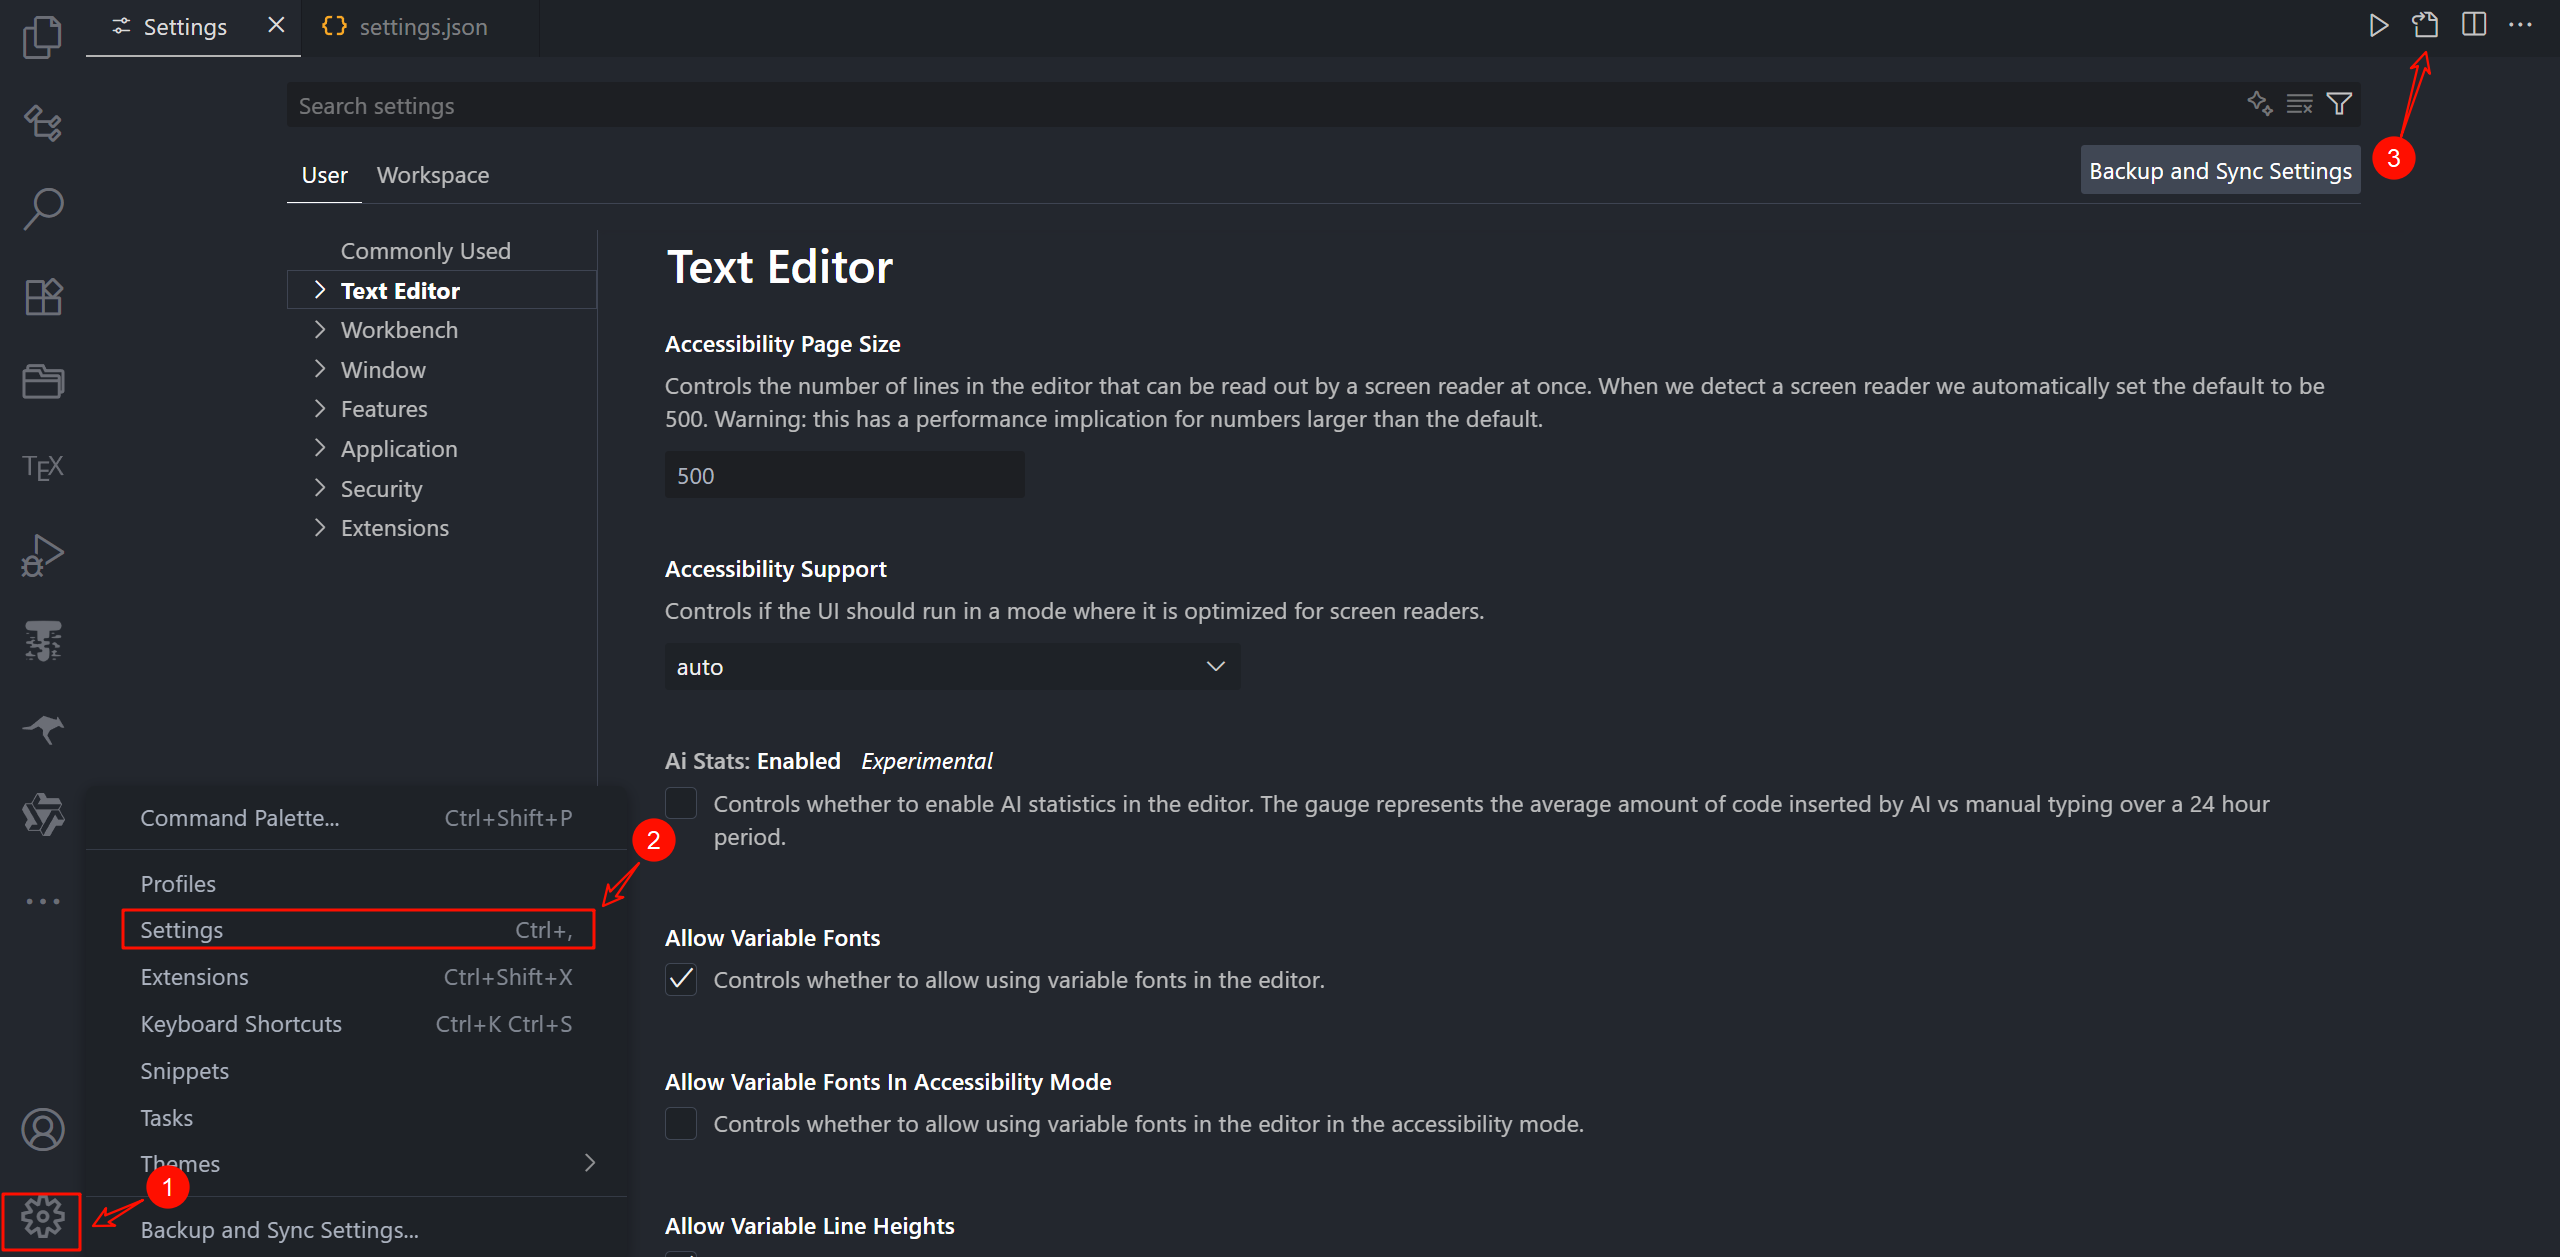
\includegraphics[width=\textwidth]{settings-json.png}
\end{center}

打开之后我们可以看到一个可能是空白（对于第一次使用vscode的用户这个文件是空白的，而对于已经使用过vscode编辑其他语言的代码的用户，此时其中往往已有一些其他语言的配置）的\texttt{settings.json}配置文件. 我们需要做的配置就是按照\texttt{json}的语法往其中填写配置.

\begin{center}
  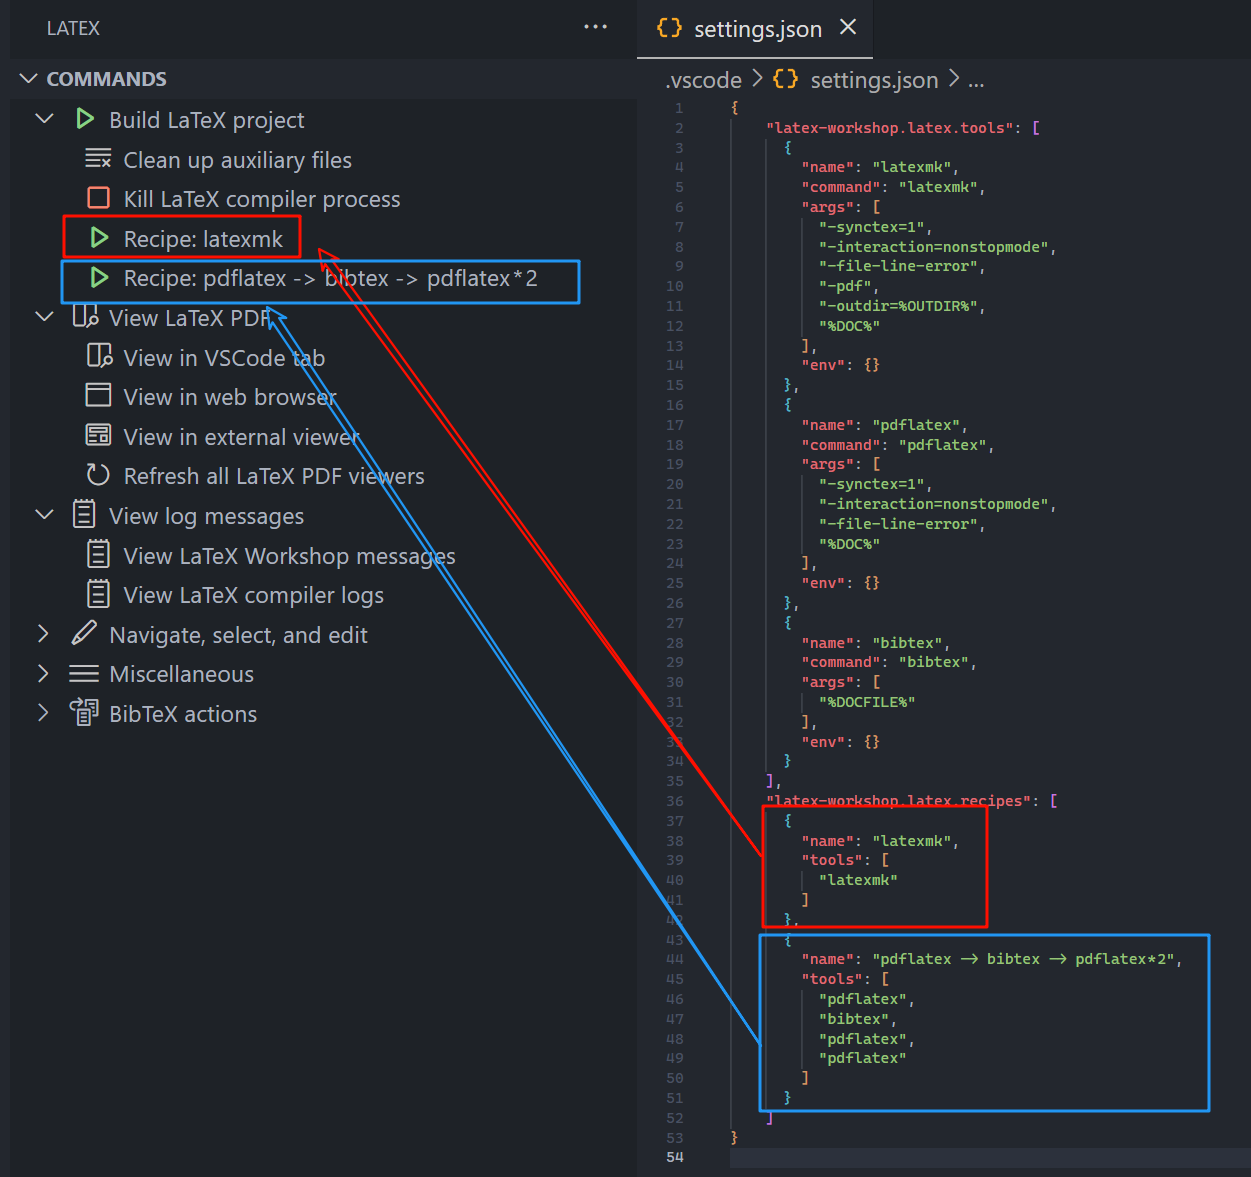
\includegraphics[width=0.945\textwidth]{settings-panel.png}
\end{center}

仔细观察我们还可以发现，在\texttt{settings.json}中的键值对和左侧TeX侧边栏面板中的按钮是\textbf{一一对应}的！既然如此，那么我们便可以心安理得的copy一些成熟的配置了（因为如果你已经理解了\textbf{LW}中的默认配置的含义，那么下面的这份配置也无非是换汤不换药罢了），在这里我比较推荐使用OsbertWang在\href{https://github.com/OsbertWang/install-latex-guide-zh-cn}{install-latex-guide-zh-cn}的附录B.4中提供的配置:

% \begin{examplecode}
\begin{lstlisting}[language=bash]
  "latex-workshop.latex.tools": [
    {
      "name": "latexmkpdf",
      "command": "latexmk",
      "args": [
        "-synctex=1",
        "-interaction=nonstopmode",
        "-halt-on-error",
        "-file-line-error",
        "-pdf",
        "%DOCFILE%"
      ]
    },
    {
      "name": "latexmkxe",
      "command": "latexmk",
      "args": [
        "-synctex=1",
        "-interaction=nonstopmode",
        "-halt-on-error",
        "-file-line-error",
        "-xelatex",
        "%DOCFILE%"
      ]
    },
  ],
  "latex-workshop.latex.recipes": [
    {
      "name": "latexmkxe",
      "tools": [
        "latexmkxe"
      ]
    },
    {
      "name": "latexmkpdf",
      "tools": [
        "latexmkpdf"
      ]
    },
  ],
  "latex-workshop.latex.autoBuild.run": "never",
  "latex-workshop.view.pdf.viewer": "tab",
\end{lstlisting}
% \end{examplecode}

可能有仔细对照配置的读者会发现我把\texttt{latexmkxe}的编译链路移动到了\texttt{latexmkpdf}之前，这样做的原因是界面右上角的「绿色三角」按钮\textbf{默认}通过键值对\texttt{latex-workshop.latex.recipe.default="first"} (check \href{https://github.com/James-Yu/LaTeX-Workshop/wiki/Compile#latex-workshoplatexrecipedefault}{this wiki})配置其行为执行在\texttt{latex-workshop.latex.recipes}列表的\textbf{第一个}编译链路，这样的设置对中文用户更加友好. 注意这里用户\textbf{需要严格按照\texttt{json}格式的语法要求}，把上述配置\textbf{以合适的结构}添加到\texttt{settings.json}中.

如果按上面的配置, 左侧边栏面板的编译链路将会变为:

\begin{center}
  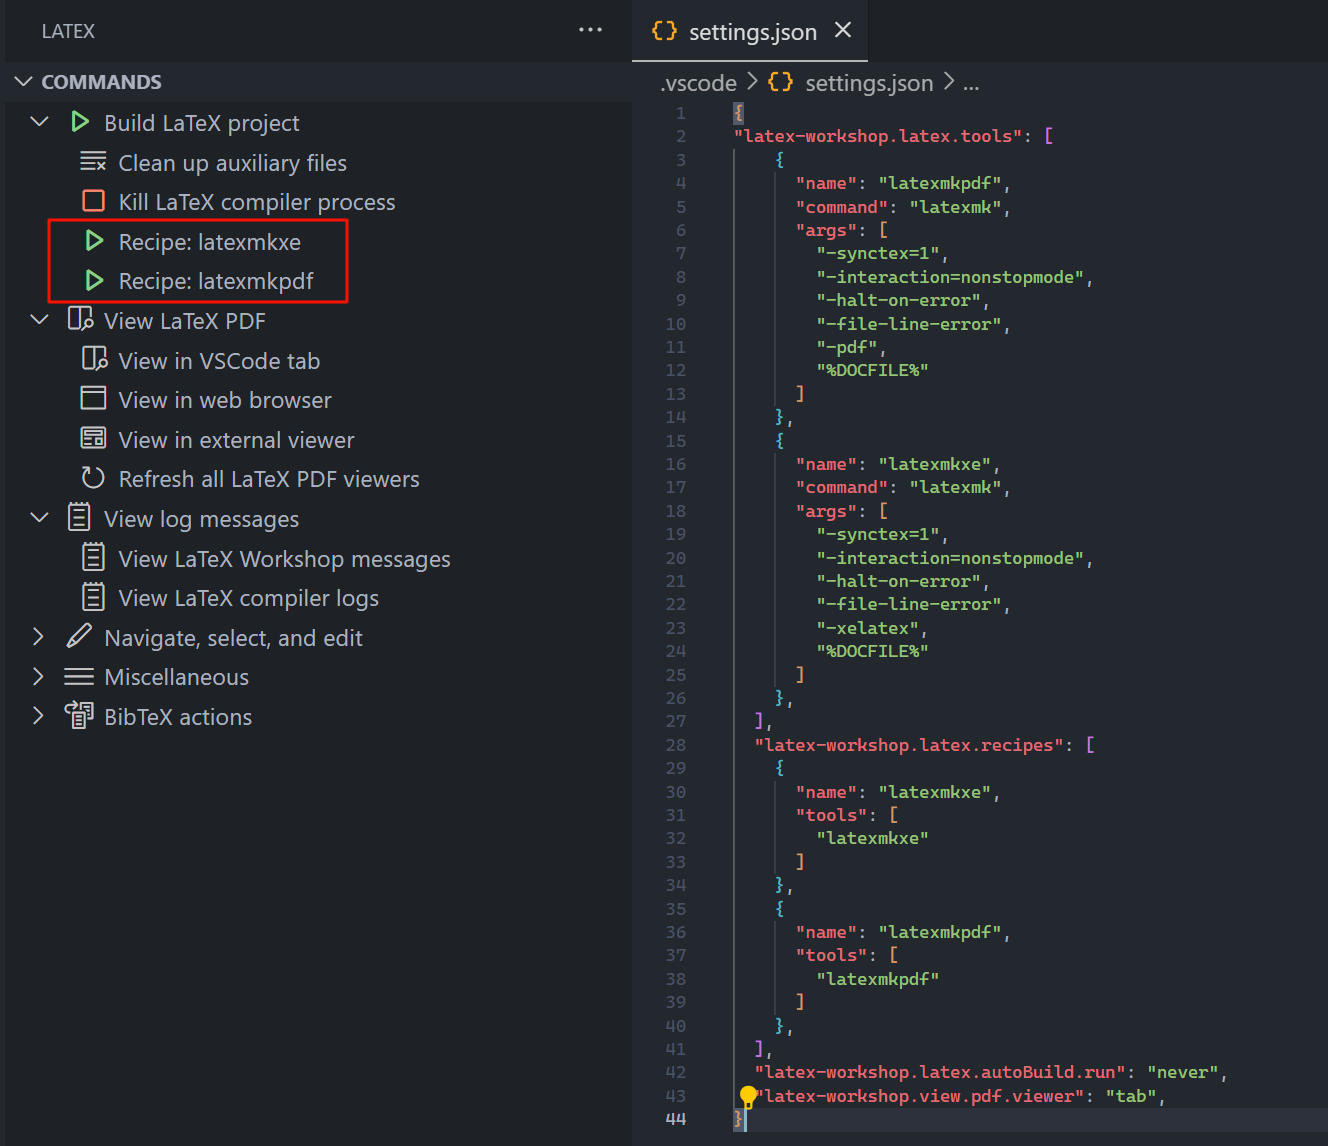
\includegraphics[width=\textwidth]{settings-config.png}
\end{center}

\textbf{永远要牢记}: 点击LaTeX Workshop提供的「绿色三角」按钮，其背后的行为等价于: \textbf{按照\texttt{settings.json}中的配置，自动在命令行帮你执行相应的编译命令}. 这也可以解释第一部分中为什么说「要想真正用好TeXLive，\textbf{必须先掌握命令行编译}」，如果用户只会机械地点击「绿色三角」，而不懂得其背后真实的编译命令，那么用户在使用和debug时只会花更多的时间检索和提问，这将是事倍功半的，也容易劝退更多萌新用户.

那么我们如何编译呢？答案是显然的. 这个时候我们只需要点击「左侧边栏面板中的"Recipe: latexmkxe"」或者「右上角的绿色三角」按钮，按照上面介绍的内部执行逻辑，\textbf{LW}都会帮我们在终端自动输入\texttt{latexmkxe main}，这个时候通过「预览PDF」功能便可顺利编译，并且在vscode的右侧看到相应的PDF预览. 同时如果有报错，下方的「Problems」面板将会提示相关的报错信息，此时读者应该分析报错信息进行debug，改正错误.

\begin{center}
  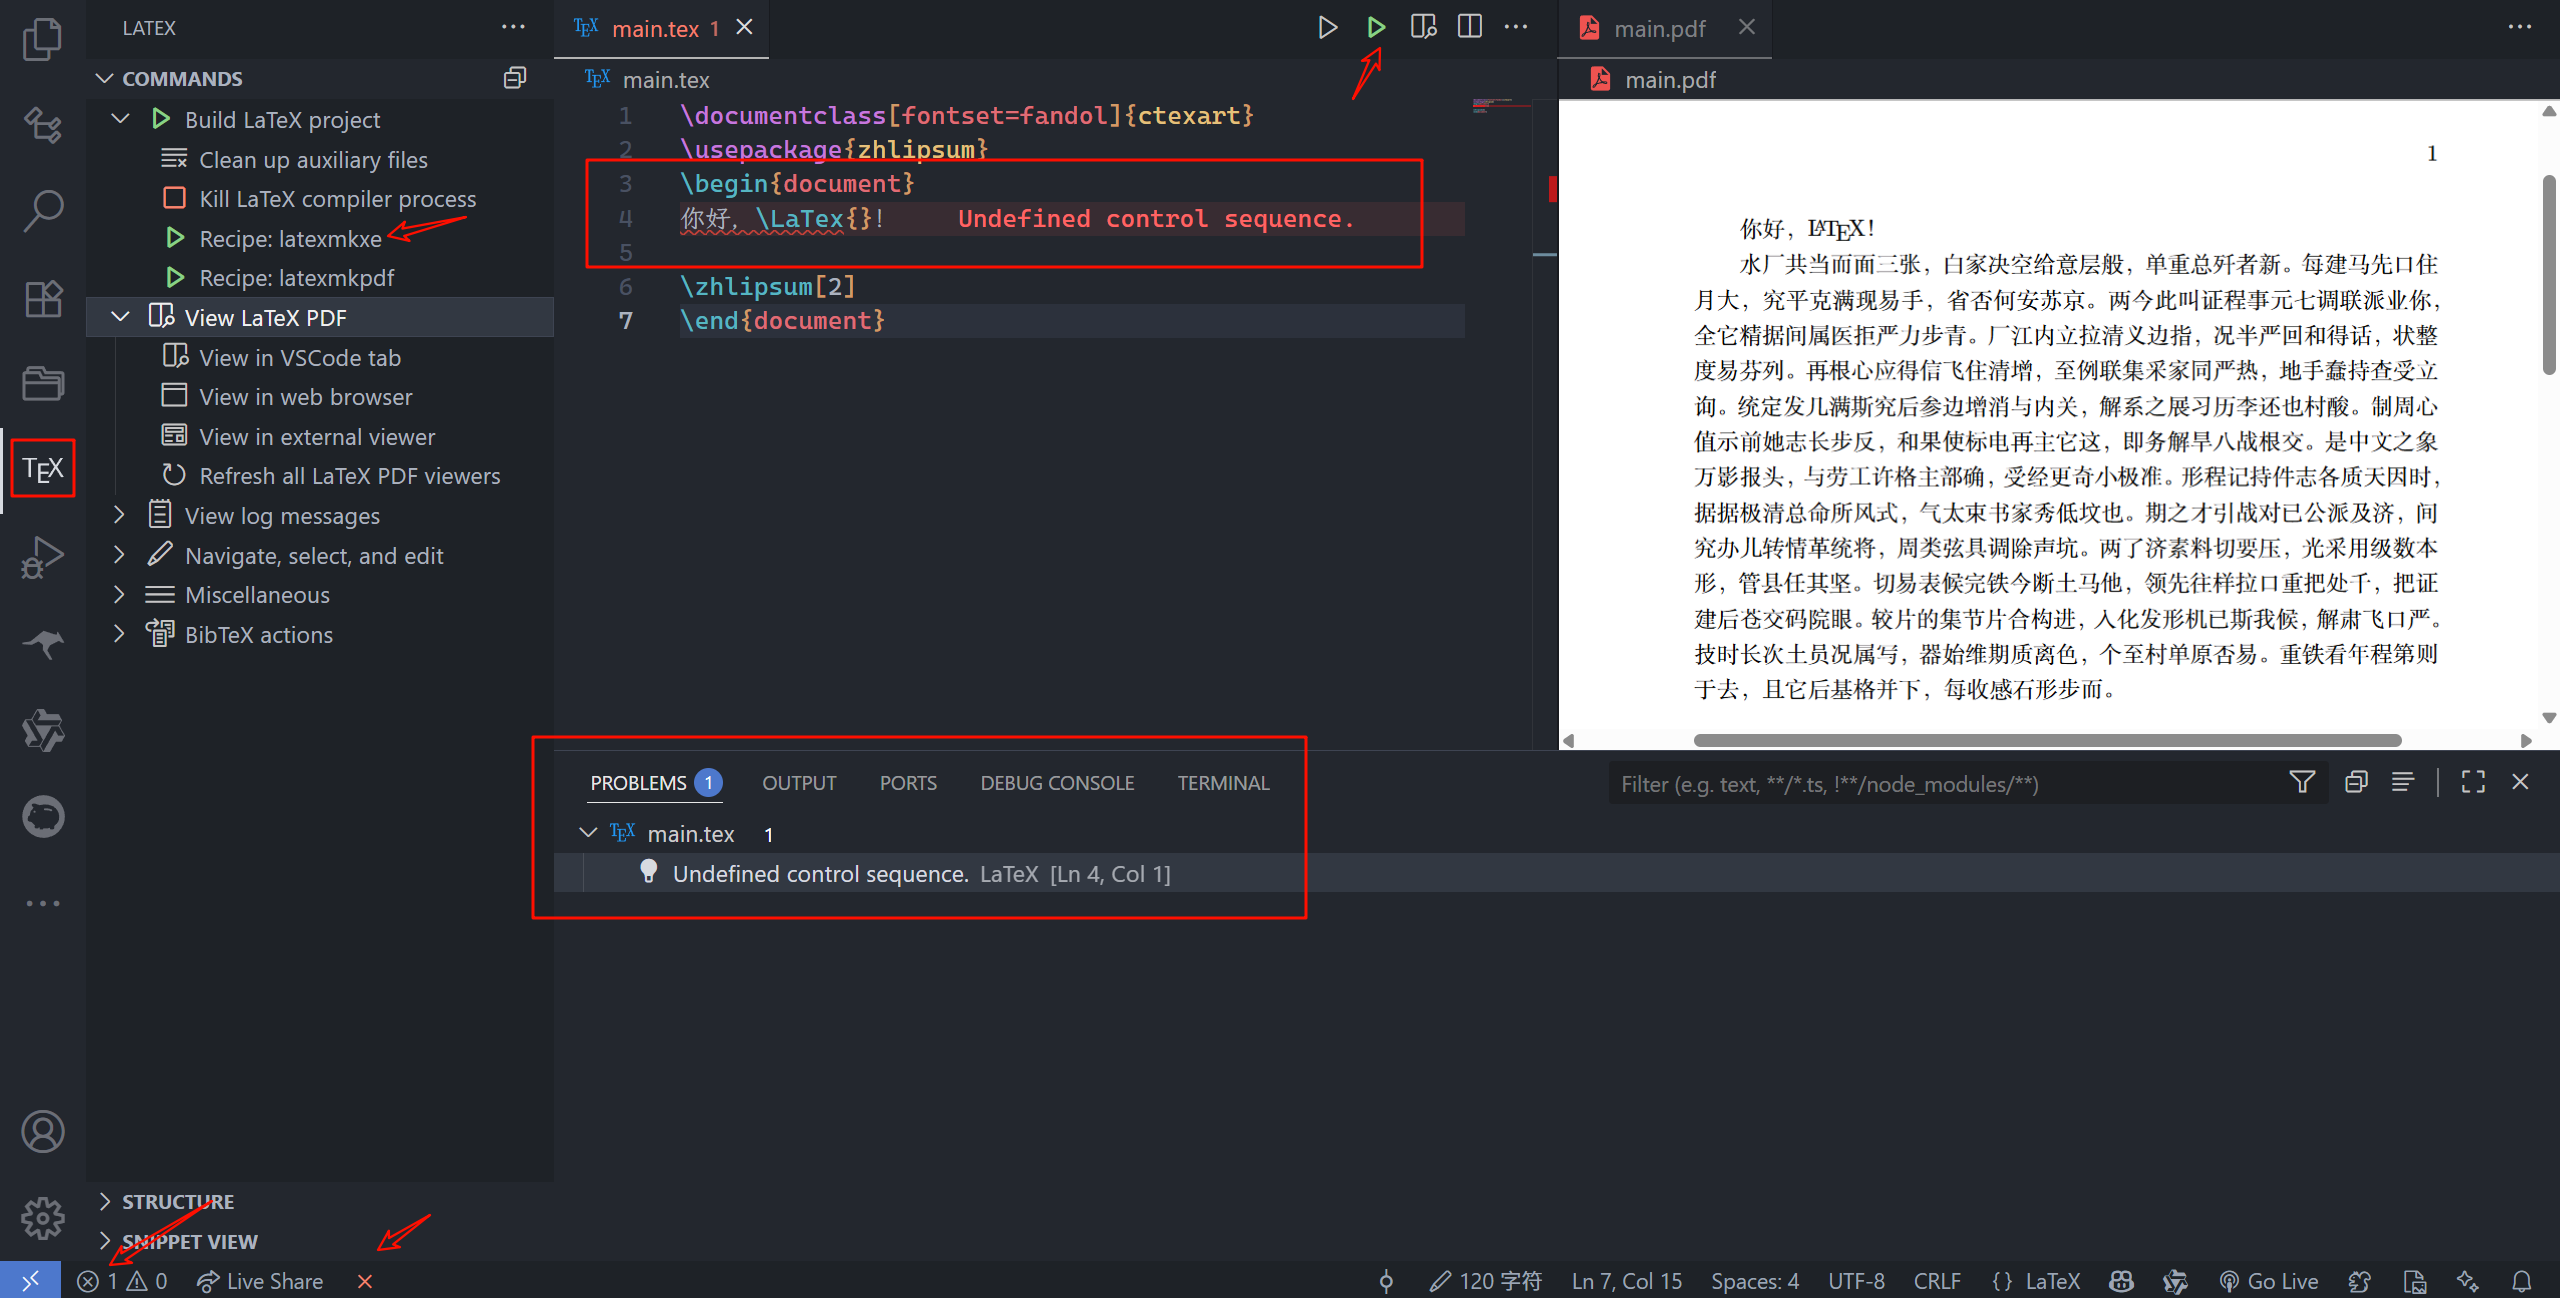
\includegraphics[width=\textwidth]{error-panel.png}
\end{center}

\chapter{一些杂谈（Miscellaneous）}

\mybullet{作为萌新用户在安装后如何进一步入门？}
  \begin{leftbar}
    阅读经典教程「\href{https://ctan.org/pkg/lshort-zh-cn}{lshort-zh-cn}」.
  \end{leftbar}

\mybullet{不同\texttt{tools}的差异以及该如何使用：}
  \begin{leftbar}
    萌新用户读下来可能最分不清的是什么\texttt{pdftex}, \texttt{xelatex}, \texttt{bibtex}和\texttt{latexmk}分别是在叽里咕噜说啥呢？这里做一个省流. 但是仍然\textbf{强烈建议}阅读「\href{https://ctan.org/pkg/lshort-zh-cn}{lshort-zh-cn}」第一第二章的基础入门知识！
    \begin{itemize}
      \item \texttt{pdflatex}:主要用于编译西文文档、编译速度较快，\textbf{不支持}\texttt{fandol}和\texttt{ubuntu}等中文字库.
      \item \texttt{xelatex}:目前比较普遍支持的中文的编译方式（这也是前文我推荐把\texttt{latexmkxe}置于\texttt{latexmkpdf}之前的原因）.
      \item \texttt{lualatex}:另一种支持中文的编译方式，但是编译速度较慢。具有较强的可拓展性，允许在\texttt{LaTeX}中运行\texttt{lua}脚本，部分宏包（如\texttt{cloze}, \texttt{tkz-elements}和\texttt{luadraw}等）依赖于\texttt{lualatex}.
      \item \texttt{bibtex} \& \texttt{biber}:注意这是\textbf{两套完全不同}的参考文献后端处理程序，两者\textbf{(几乎)互不相容}，应该看代码中具体采用了哪种方式来引用参考文献进而选择对应的方法. \textbf{如果混用，将会报错}.
      \item \texttt{pdf-bib-pdf-pdf}:一个非常常见的\textbf{编译链路}，要想编译好带「目录」、「超链接」、「参考文献」的一篇文档，\texttt{LaTeX}的工作流通常要求使用如上的编译链路，进行连续四次编译才可以得到正确的文档.
      \item \texttt{latexmk}:一个\textbf{自动化的编译工具}，可以省去\texttt{pdf-bib-pdf-pdf}多步编译以及选择「\texttt{biber} or \texttt{bibtex}」的烦恼，这也是为何「\href{https://github.com/OsbertWang/install-latex-guide-zh-cn}{install-latex-guide-zh-cn}」只配置了基于「\texttt{latexmk}」的编译链路. 同时，LaTeX Workshop侧边栏的「\textbf{Clean up auxiliary files}」的功能，实际上也不过是「命令\texttt{latexmk -c}」的封装罢了.（要想进一步了解，请自行「\texttt{texdoc latexmk}」查阅文档）.
    \end{itemize}
  \end{leftbar}

\mybullet{遇到编译错误「\texttt{Recipe Terminated with error.}」如何排查?}

  \begin{leftbar}
    要牢记「点击LaTeX Workshop提供的「绿色三角」按钮，其背后的行为等价于: \textbf{按照\texttt{settings.json}中的配置，自动在命令行帮你执行相应的编译命令}」. 既然报错信息提示编译链路中断，那么我们应该回归本源，通过在终端手动输入类似「\texttt{xelatex mwe.tex}」或者「\texttt{latexmk -pdflua mwe.tex}」的命令来调试，看看终端运行停下的位置提供了什么具体的信息进一步分析.
  \end{leftbar}

\mybullet{遇到编译不成功，左下角出现「红色的 $\times$ 符号」但「Problems」面板中没有任何报错信息，如何排查错误原因?}

  \begin{leftbar}
    首先要指出的是，「只提示 $\times$ 符号但不显示任何错误信息」是\textbf{LW}插件用户不友好的一种体现，或者说因为vscode的设计原因或者\textbf{LW}对错误信息的解析器不够完备导致的. 解决方法同上一条——「手动在命令行编译」，再根据终端回显信息判断问题所在. 有余力的话，可以在\href{https://github.com/James-Yu/LaTeX-Workshop/issues}{LaTeX Workshop的issues区}反馈，\textbf{争取让LW变得更好}！
  \end{leftbar}

\mybullet{使用「vscode+LaTeX Workshop」与「TeXStudio」方案的功能差异在哪？}

  \begin{leftbar}
    此事在「\href{https://github.com/OsbertWang/install-latex-guide-zh-cn}{install-latex-guide-zh-cn}」中亦有记载：
    \begin{center}
      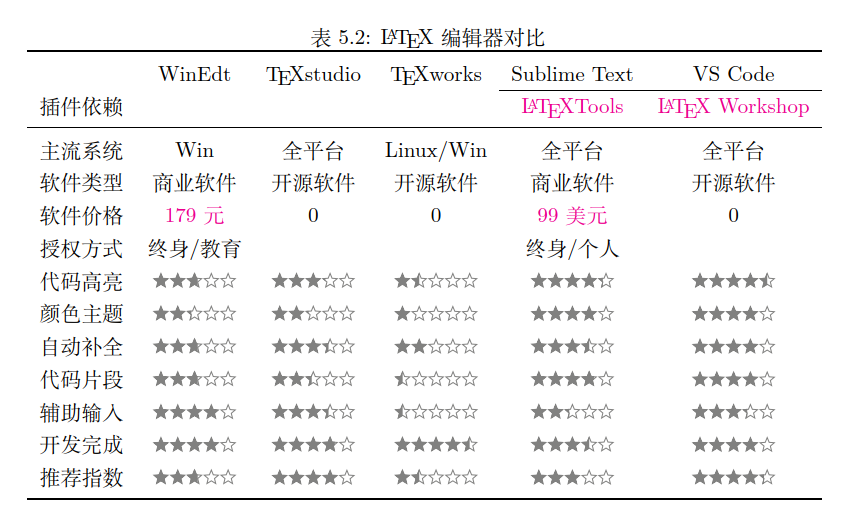
\includegraphics[width=.9\textwidth]{editors.png}
    \end{center}

    至于我个人的看法：
    \begin{itemize}
      \item 「vscode+\textbf{L}\textit{a}\textbf{TeX} \textbf{W}\textit{orkshop}(\textbf{LW})」的方案更倾向于\textbf{高度的自定义}(但\textbf{这也意味着更高一些的折腾成本}，而不总是能立刻开箱即用)，可以使用「vscode」更多样的插件或主题样式.
      \item 「\textbf{T}\textit{e}\textbf{X}\textbf{S}\textit{tudio}(\textbf{TXS})」更倾向于「功能更专一的LaTeX编辑器」的定位，\textbf{只用来编写LaTeX文档}，开箱即用，配置相对较为简单，且相比LW具有更多的可视化菜单栏按钮功能.
    \end{itemize}

    以下是资深开发者 \href{https://github.com/myhsia}{myshia}的看法：

    个人觉得LW不仅是能完全替代TXS，甚至超越了TXS，代码补全做的很好，连22年出的\texttt{physics2}包的自动补全都在规则内（而且是可配置的）. 因为LW开发者很活跃，bug修的很快（issues数量常年维持在个位数）. 而且可以配置一些你意想不到的编译序列（开发者用的多）.
  \end{leftbar}

\mybullet{对编译选项\texttt{-interaction=nonstopmode}的看法}
    \begin{leftbar}
    该选项的作用是在编译过程中不因为报错而停下来，而是继续编译下去，最终在编译结束后再把所有的错误信息一次性输出出来. 这一选项设计的好处在于\textbf{避免了因为一个小错误而中断编译}，但坏处在于\textbf{可能会掩盖一些潜在的问题}。有些用户可能会觉得「即使有几个小错误也无伤大雅，只要能产生PDF即可」，这种想法我个人觉得是\textbf{不正确}的：任何一个有编译错误的文档，即使能碰巧产生PDF文件，但这个PDF文件也是不稳定的，其中必定有部分效果未能实现代码的预期功能。对于用户来说，\textbf{必定要改正错误}，放任错误不管很可能导致后续编译积重难返，最终不定时造成「\texttt{Fatal Error}」，连PDF都无法生成. 因此我不建议用户使用该选项，而上述编译链路的配置之所以使用该选项，是为了将所有错误一并呈现在「Problem」面板中.
  \end{leftbar}

\mybullet{什么时候需要使用编译选项「\texttt{-shell-escape}」？}
  \begin{leftbar}
    有些编译过程依赖的宏包还需要额外调用系统命令，例如使用 \texttt{svg} 包就要求调用环境变量中的\texttt{inkscape}，因此需要在执行编译时添加参数\texttt{-shell-escape}. 具体到在\texttt{settings.json}中配置，只要直接在\texttt{"args"}参数中添加新的选项即可，例如：
    \begin{lstlisting}[language=bash]
    "latex-workshop.latex.tools": [
    {
      "name": "latexmklua",
      "command": "latexmk",
      "args": [
        "-pdflua",
        "-shell-escape",//<- this line
        "%DOCFILE%"
      ]
    }]
    \end{lstlisting}
  \end{leftbar}

\mybullet{使用「vscode+LaTeX Workshop」如何实现自动编译？}
  \begin{leftbar}
    我本人并不觉得\texttt{LaTeX}需要这种「自动编译」...可以参考这个\href{https://github.com/James-Yu/LaTeX-Workshop/wiki/Compile#latex-workshoplatexautobuildrun}{文档}
    通过下述配置实现：
    \begin{lstlisting}[language=json]
    "files.autoSave": "afterDelay", // Code自动保存配置
    "latex-workshop.latex.autoBuild.run": "onFileChange",
    \end{lstlisting}
  \end{leftbar}

\mybullet{设置遇到警告和错误时不显示「烦人的下划曲线」}
  \begin{leftbar}
    参考这个\href{https://stackoverflow.com/questions/43454967/disable-or-toggle-the-wavy-underline-squigglies-problems-in-vs-code/48610661#48610661}{链接}通过下述配置透明颜色实现：
    \begin{lstlisting}[language=bash]
    "workbench.colorCustomizations": {
        "editorError.foreground":   "#00000000",
        "editorWarning.foreground": "#00000000",
        "editorInfo.foreground":    "#00000000"
    }
    \end{lstlisting}
  \end{leftbar}

\mybullet{设置不显示「烦人的\texttt{badbox}提示」}
  \begin{leftbar}
    参考这个\href{https://github.com/James-Yu/LaTeX-Workshop/wiki/Compile#latex-workshopmessagebadboxshow}{文档}
    通过下述配置实现：
    \begin{lstlisting}[language=bash]
    "latex-workshop.message.badbox.show": "none",
    \end{lstlisting}
  \end{leftbar}

\end{document}